%\newpage
\chapter{Beschreibung der BJT-Messungen}
\label{sec:BJTmeasurements}

\begin{figure}[H]
  \begin{subfigure}[b]{9cm}
    \centering
    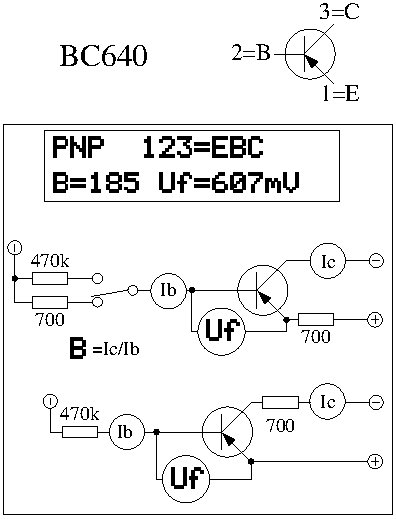
\includegraphics[width=9cm]{../FIG/BJT_BC640.pdf}
    \caption{PNP}
    \label{fig:BJT-PNP}
  \end{subfigure}
  ~
  \begin{subfigure}[b]{9cm}
    \centering
    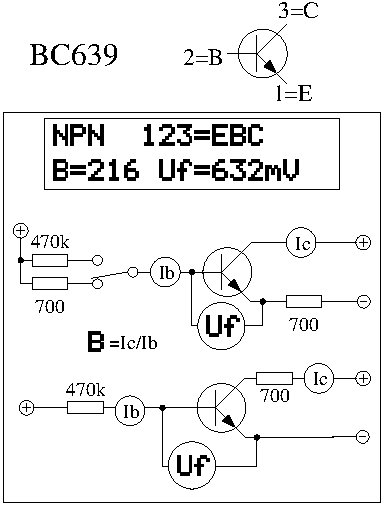
\includegraphics[width=9cm]{../FIG/BJT_BC639.pdf}
    \caption{NPN}
    \label{fig:BJT-NPN}
  \end{subfigure}
  \caption{Bipolare Silizium Transistoren}
\end{figure}


\begin{figure}[H]
\centering
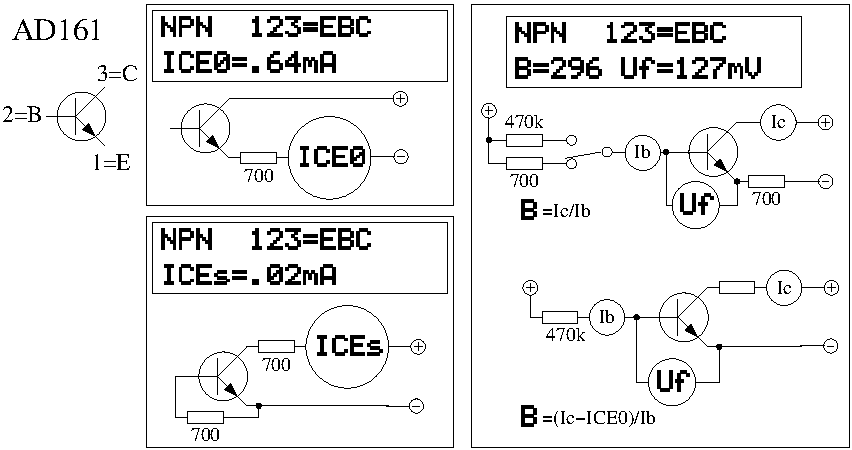
\includegraphics[]{../FIG/BJT_AD161.pdf}
\caption{NPN-Germanium-Transistor}
\label{fig:BJT-NPN-Ge}
\end{figure}


\begin{figure}[H]
\centering
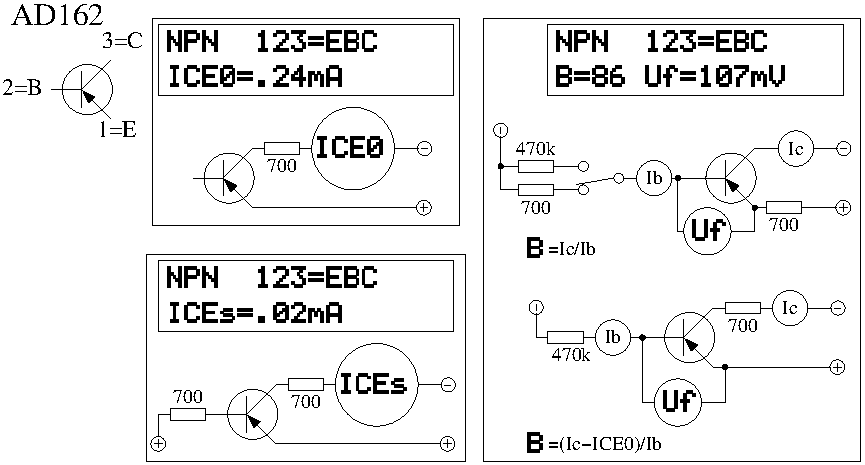
\includegraphics[]{../FIG/BJT_AD162.pdf}
\caption{PNP-Germanium-Transistor}
\label{fig:BJT-PNP-Ge}
\end{figure}

\begin{figure}[H]
  \begin{subfigure}[b]{9cm}
    \centering
    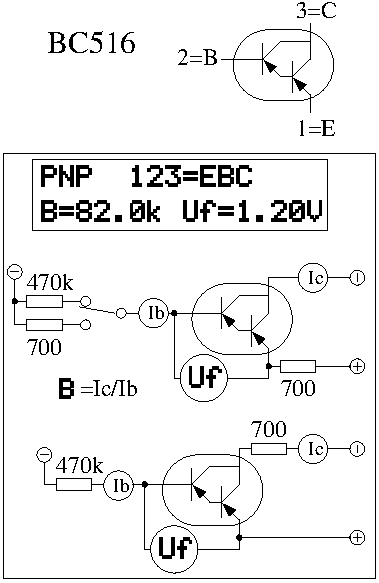
\includegraphics[width=9cm]{../FIG/BJT_BC516.pdf}
    \caption{PNP}
    \label{fig:BJT-PNP-Darl}
  \end{subfigure}
  ~
  \begin{subfigure}[b]{9cm}
    \centering
    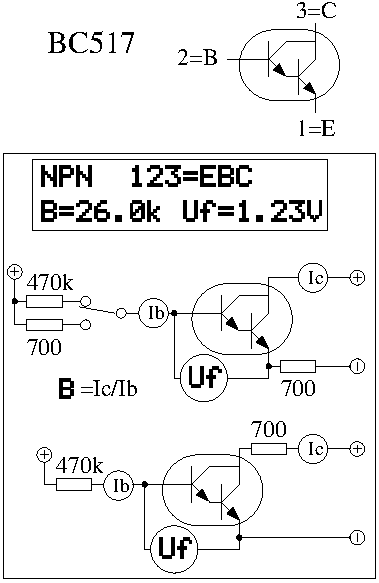
\includegraphics[width=9cm]{../FIG/BJT_BC517.pdf}
    \caption{NPN}
    \label{fig:BJT-NPN-Darl}
  \end{subfigure}
  \caption{Silizium Darlington-Transistoren}
\end{figure}

\begin{figure}[H]
\centering
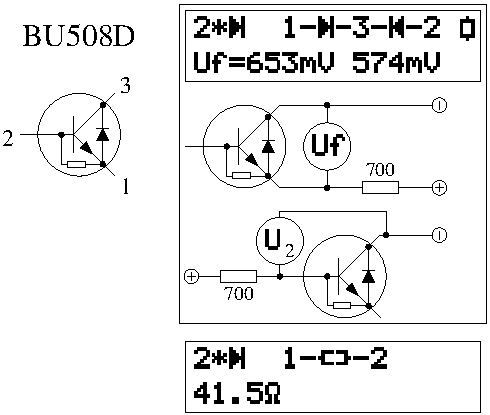
\includegraphics[]{../FIG/BJT_BU508D.pdf}
\caption{NPN-Transistor mit Diode und Widerstand}
\label{fig:BJT-NPN-Di-R}
\end{figure}

\begin{figure}[H]
  \begin{subfigure}[b]{9cm}
    \centering
    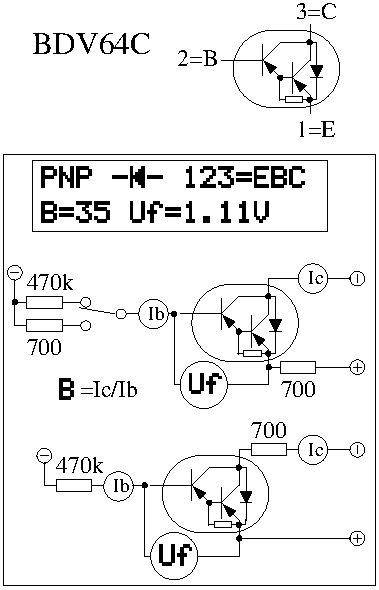
\includegraphics[width=9cm]{../FIG/BJT_BDV64.pdf}
    \caption{PNP}
    \label{fig:BJT-PNP-Darl-R-D}
  \end{subfigure}
  ~
  \begin{subfigure}[b]{9cm}
    \centering
    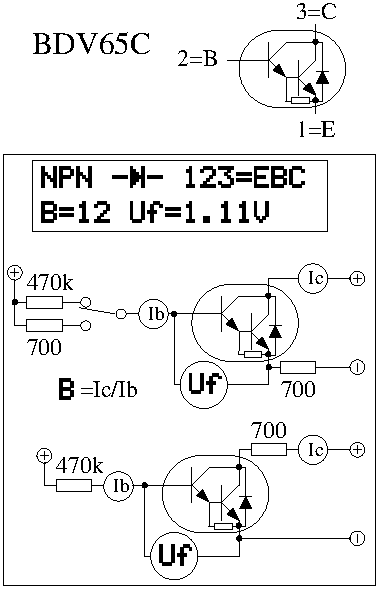
\includegraphics[width=9cm]{../FIG/BJT_BDV65.pdf}
    \caption{NPN}
    \label{fig:BJT-NPN-Darl-R-D}
  \end{subfigure}
  \caption{Silizium Darlington-Transistoren}
\end{figure}
